\chapter{Construção da Ferramenta \tjscraper~\label{chp:construção-da-ferramenta}}

A ferramenta construída neste trabalho, nomeada \textbf{\tjscraper}, foi
produzida para ser capaz de extrair com qualidade satisfatória os dados de
processos dos Tribunais de Justiça (TJs), tendo no momento implementada a
extração de dados especificamente do TJ do Rio de Janeiro (TJ-RJ). As
estratégias empregadas, portanto, levam em conta acessos que todos os acessos
serão ao TJ-RJ, ainda que visando a possibilidade de serem aplicadas às páginas
dos TJs dos demais estados.

Conforme critérios próprios deste trabalho, a qualidade dos dados extraídos
será considerada satisfatória se:

\begin{itemize}
    \item Puderem ser trivialmente exportados para um formato legível para quem
        não conheça o funcionamento interno da ferramenta. Tal formato pode ser
        um formato de arquivo como uma planilha XLSX ou uma visualização em
        tabela em HTML;
    \item Possuírem campos úteis para análises tanto individuais quanto
        estatísticas dos processos como nomes das partes, assunto, data de
        abertura e última movimentação;
    \item A forma como os dados estão guardados viabilize realizar consultas
        personalizadas neles, tais como busca por assunto.
\end{itemize}

\section{Ferramentas utilizadas~\label{section:ferramentas-utilizadas}}

\textcolor{blue}{--->> O que estás propondo para descrição de ferramentas
(Scrapy e SQLLite) será um pequeno parágrafo de uma Seção chamada "Ferramentas
utilizadas" no capítulo de construção da ferramenta. Não vais descrever nenhuma
delas com detalhes, pois são ferramentas simplesmente usadas para contruíres
teu trabalho. Isso não se detalha porque não são "conceitos". Ferramentas mudam
de versão, saem de linha, ficam obsoletas, perdem valor, etc, portanto, não se
descrevem em detalhes.}

\todo{%
    Esta seção deve ser uma descrição das ferramentas mais relevantes que foram
    \textit{utilizadas} no trabalho, i.e. as dependências (bibliotecas,
    linguagem de programação).
}
\begin{todolist}
    \item Python 3.10 (listar motivos: incluir que não precisa de otimizações
        agressivas do compilador pois o gargalo é IO de rede). Frisar as
        palavras \textbf(``Critérios Técnicos'').
    \item Scrapy
    \item SQLite
    \item \ldots
\end{todolist}

\section{Organização geral}

\begin{todolist}
    \item Diagramar módulos;
\end{todolist}

A ferramenta foi projetada como uma biblioteca de \textit{software} acompanhada
de duas interfaces de usuário~\footnote{Nesta seção, ``usuário'' refere-se a
alguém que não esteja utilizando a ferramenta como uma biblioteca de software,
e sim como aplicação.}: uma aplicação de Interface de Linha de Comando
(ILC\footnote{Comumente referenciado com a sigla em inglês ``CLI'', de
``Command Line Interface''.}) e uma aplicação de servidor Web.

A ILC tem como objetivo permitir o uso de boa parte dos diferentes recursos da
biblioteca em um terminal para a execução tarefas pontuais, como exibir
informações sobre estado atual da \textit{cache}, iniciar um processo de
extração, ou mesmo iniciar uma instância de servidor Web da ferramenta para
fins de desenvolvimento.

O servidor Web é destinado ao usuário que queira uma interface de simples
acesso e uso da ferramenta, primariamente focando na obtenção de dados dos TJs
com os recursos que não estejam disponíveis nas páginas oficiais dos TJs
(descritos na~\Cref{sec:Motivação-e-Contexto}), tendo em mente como público
alvo jornalistas.

\section{Estratégias de extração}

O TJ-RJ possui rotas e subdomínios que dão acesso aos mesmos dados de processos
por formatos de apresentação diferentes. Foram elaboradas estratégias para
extrair dados da rota que os fornece em formato HTML, conhecida antes da
produção efetiva da ferramenta, e da que os fornece em formato JSON, encontrada
durante o processo de produção e portanto implementada posteriormente. O
formato HTML é apresentado como uma página de consulta para um usuário humano,
enquanto o formato JSON é um conjunto de rotas que implementam uma API Web.

Para a produção desta ferramenta não foi encontrada uma forma de se obter todos
os processos de maneira direta, como uma lista de números de processo
existentes ou uma tabela de registros no TJ-RJ. A estratégia adotada para isso,
então, foi descobri-los exaurindo as possibilidades de valores de entrada de
algum dos tipos de busca disponíveis nos portais do TJ-RJ. Analisando as
dificuldades existentes em cada um dos tipos
(\Cref{tbl:dificuldades-tipos-de-busca}), foi escolhido o campo de busca por
número do processo por conta do domínio de valores válidos ser limitado e
conhecido: números de processos são dados seguindo os formatos numéricos fixos
\textbf{unificado} e \textbf{antigo}.

\begin{table}[tb]
    \centering
    \begin{tabular}{lp{0.65\textwidth}}
        \toprule
        Tipo de busca & Dificuldades \\
        \midrule
        Por Número & Número alto de combinações possíveis (para cada ano,
                     $10^{7} \times |O|$ tanto para numeração unificada quanto
                     antiga, em que $|O|$ é a quantidade de unidades de origem
                     do TJ em questão). \\
        Por Nome & Inviável. Demanda conhecer todos os nomes existentes em processos. \\
        Por OAB & Sem garantia de cobertura completa. \\
        Por Nome do Advogado & Inviável. Demanda conhecer todos os nomes existentes em processos. \\
        Por CPF / CNPJ & Número alto de combinações possíveis (em um sequenciamento ingênuo, $10^{11}$ para CPF e $10^{14}$ para CNPJ). \\
        Por Protocolo & Sem garantia de cobertura completa. \\
        Por Sentença & Sem garantia de cobertura completa. \\
        \bottomrule
    \end{tabular}
    \caption{%
        Dificuldades encontradas para se exaurir as possibilidades de valores
        de entrada para cada um dos campos de busca permitidos pelo TJ-RJ.
    }
    \label{tbl:dificuldades-tipos-de-busca}
\end{table}

O \textbf{unificado} (também referenciado como ``numeração única'') é universal
para todos os TJs, padronizado pelo CNJ
\cite{spec:cnj-numeração-única,spec:cnj-numeração-única-resolução} e segue o
padrão ``NNNNNNN-DD.AAAA.J.TR.OOOO'', em que ``NNNNNNN'' é um número sequencial
e único dado a cada processo, ``DD'' são os dígitos verificadores validados
pelo algoritmo Módulo 97 Base 10~\cite{spec:iso-modulo-97}, ``AAAA'' indica o
ano de distribuição, ``J'' identifica o órgão ou segmento do Poder Jucidiário
conforme a relação enumerada em~\cite{spec:cnj-numeração-única-resolução}
Artigo 1º \S 4º, ``TR'' é uma subclassificação do órgão/segmento e indica qual
o Tribunal em questão (19 para o TJ-RJ) e ``OOOO'' é o código de a qual das
unidades de origem (específicas para cada TJ) o processo se refere.

O \textbf{antigo} é o formato de numeração próprio de uso interno que cada TJ
define para si. O do TJ-RJ segue o padrão ``AAAA.OOO.NNNNNN-N'' em que ``AAAA''
indica o ano de distribuição, ``OOO'' é o código da unidade de origem e cada
``N'' restante é um dígito de 0 a 9. Diferentemente da numeração unificada, os
campos com ``N'' não são designados de forma serial, podendo haver sequências
intercaladas de números que não correspondam a processos válidos.

Considerando ambos os formatos de numeração, para se exaurir as entradas
possíveis é possível fixar um ano e um TJ (neste caso, o TJ-RJ) --- o que
também implica em fixar o segmento em 8 (valor para a categoria ``Justiça dos
Estados e do Distrito Federal e Territórios'') --- e variar os dígitos para os
demais campos. No caso da unidade de origem, é possível se basear em uma lista
conhecida~\cite{spec:tjrj-codigos-unidades-de-origem}, o que reduz o número de
entradas a se testar, e por fim os dígitos de verificação podem ser calculados
a partir de uma combinação dos demais campos, não interferindo na quantidade de
entradas testadas.

Apesar de supostamente o número de entradas a se testar para ambos os tipos de
numeração ser o mesmo, a preferência foi dada à \textbf{numeração unificada}
para descoberta de processos válidos tanto pelo caráter de padronização
nacional, abrindo espaço para facilitar a adaptação de seu uso em outros TJs
além do TJ-RJ do ponto de vista de implementação da ferramenta, quanto por
algumas unidades de origem que possuem seu código de 4 dígitos não terem um
espelho com 3 dígitos~\cite{spec:tjrj-codigos-unidades-de-origem}. Além disso,
há também o fator de serialidade do campo ``N'' na numeração unificada, que
permite saber que a partir do primeiro processo inexistente encontrado a busca
pode ser finalizada concluindo-se que todos os processos daquele TJ registrados
até o momento no sistema foram encontrados.

Os demais métodos de busca, como via nome das partes, possuem uma abrangência
de valores muito grande e difícil de se conhecer em sua totalidade ou, nos
casos como a busca por Sentença, não são capazes de, mesmo exauridas todas as
combinações de valores de entrada, dar acesso a todos os processos registrados
(visto que nem todo processo possui uma sentença).

\subsection{Estratégia inicial: extração HTML}

Os resultados de consulta processual do TJ-RJ em HTML são os das requisições
feitas ao subdomínio \url{ww4.tjrj.jus.br}. Em uma URL de visualização de um
processo um válido~\footnote{Exemplo de URL de processo válido:
\url{http://www4.tjrj.jus.br/consultaProcessoWebV2/consultaProc.do?numProcesso=2021.004.015548-9}.}
nesse subdomínio (\Cref{fig:exemplo-pagina-ww4}), o parâmetro de URL
(\textit{query string}) \texttt{numProcesso} identifica o número do processo na
numeração antiga. A estratégia de extração dos processos disponibilizados por
esse subdomínio é efetuar requisições para a mesma URL variando apenas esse
parâmetro com um número de processo diferente utilizando a numeração
\textbf{antiga}. Cada requisição pode retornar uma página de processo válido,
inexistente~\footnote{Exemplo de URL de processo inexistente:
\url{http://www4.tjrj.jus.br/consultaProcessoWebV2/consultaProc.do?numProcesso=2020.004.015548-9}.},
de numeração inválida~\footnote{Exemplo de URL de processo inválido:
\url{https://www4.tjrj.jus.br/consultaProcessoWebV2/consultaMov.do?numProcesso=0}.}
ou de Captcha (caso esteja fora do horário noturno).

No caso de páginas de processo válidos, os campos que compõem os dados de um
processo estão todos na mesma página bastando então \textit{parsear} seu código
HTML. Já as páginas de erro são identificáveis ora pelo seu título e ora pelo
conteúdo com textos como ``Erro'' e ``Parâmetro Incorreto''
(\Cref{fig:exemplo-tjrj-pagina-erro}).

Por fim, ainda que o subdomínio ww4 também permita a busca por numeração única,
ao acessar o resultado de um processo válido se chega à mesma página da busca
por numeração antiga com o valor do parâmetro de URL \texttt{numProcesso}
também na numeração antiga, e portanto não bastaria apenas variar o valor desse
parâmetro com testes no formato da numeração única. É possível, contudo,
aplicar a mesma tática de requisições em duas etapas descrita
na~\Cref{sub:estrategia-api-json}.

\begin{figure}[H]
    \centering{}
    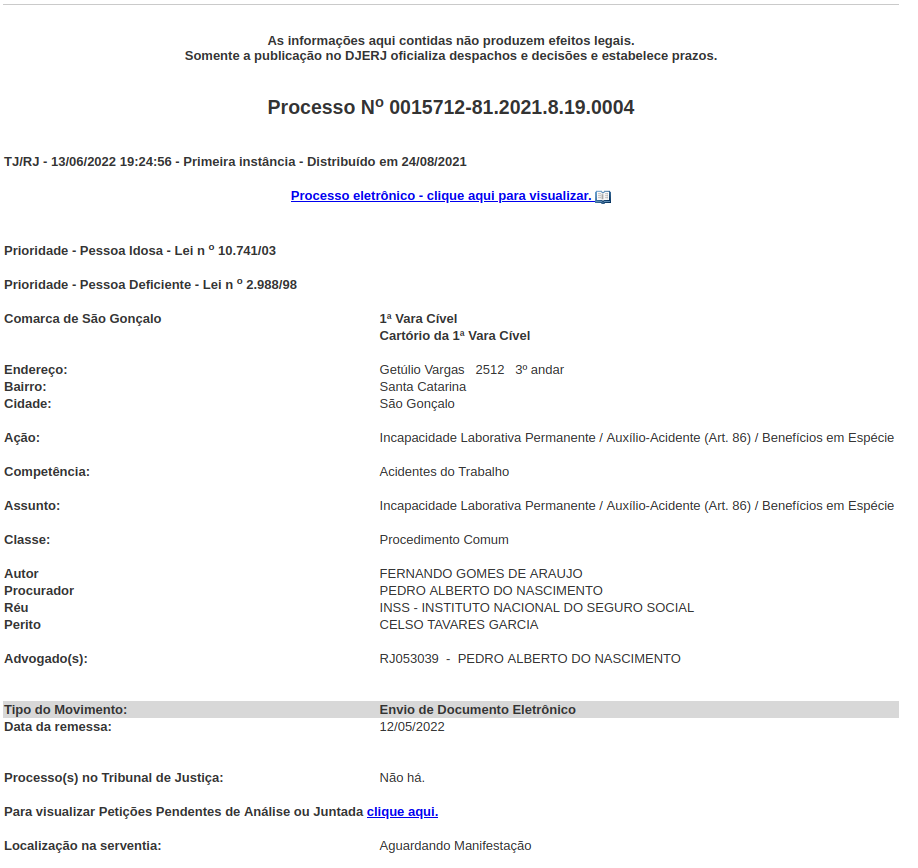
\includegraphics[width=0.8\textwidth,keepaspectratio]{img/exemplo-resultado-consulta-publica-1.png}
    \caption{%
        Página de resultado da consulta pública para o processo válido de
        número 2021.003.015548-9 (numeração antiga).
    }
    \label{fig:exemplo-pagina-ww4}
\end{figure}

\begin{figure}[H]
    \centering{}
    
\includegraphics[width=0.8\textwidth,keepaspectratio]{img/exemplo-tjrj-pagina-erro}
    \caption{%
        Página de resultado da consulta pública para um número inválido de processo.
    }
    \label{fig:exemplo-tjrj-pagina-erro}
\end{figure}

\subsection{Estratégia alternativa: varredura com API JSON\label{sub:estrategia-api-json}}

\begin{todolist}
    \item Explicar rapidamente sobre a filtragem dos campos;
\end{todolist}

\urldef\urlConsultaJson\url{https://www3.tjrj.jus.br/consultaprocessual/#%2Fconsultapublica%23porNumero=}

No subdomínio \url{ww3.tjrj.jus.br}, há uma página de
busca~\footnote{\urlConsultaJson} semelhante à oferecida no subdomínio
\url{ww4.tjrj.jus.br}, também fornecendo os dados em HTML. A diferença está que
em vez de o servidor responder com o HTML completo e pronto para o lado cliente
renderizar como uma página nova (que é o caso do subdomínio ww4), no subdomínio
ww3 ao se acionar o botão de busca o cliente envia uma requisição AJAX para uma
API do servidor, que responde com um objeto JSON com os dados do processo e
então o HTML é atualizado no lado cliente de forma dinâmica. A estratégia então
nesse caso passa a ser trivial: a partir do número de um processo, enviar uma
requisição para a tal API e, com os dados de um processo em JSON, basta
investigar quais os campos retornados, filtrar os de interesse e exportar da
forma desejada.

A API do servidor do TJ-RJ possui rotas específicas para consultas pela
numeração unificada~\footnote{Rota para consulta pela numeração unificada:
\url{https://www3.tjrj.jus.br/consultaprocessual/api/processos/por-numeracao-unica}}
e pela antiga~\footnote{Rota para consulta pela numeração antiga:
\url{http://www3.tjrj.jus.br/consultaprocessual/api/processos/por-numero/publica}},
ambas respondendo com dados de um processo através de requisições POST
utilizando \textit{query strings} para especificar os parâmetros de busca.
Os tipos de resultados de ambas as rotas encontrados durante a construção desta
ferramenta estão expostos na~\Cref{tbl:respostas-ww3}.

\begin{todolist}
    \item Passar a parte de implementação para o capítulo de implementação;
    \item Comentar que na numeração única as respostas são listas conforme
        processos em instâncias diferentes.
    \item Explicar as requisições em 2 etapas.
\end{todolist}

\begin{table}[htb]
    \tiny
    \centering
    \begin{tabular}{lp{0.55\textwidth}}
        \toprule
        \multicolumn{2}{c}{Respostas comuns às consultas por numeração antiga e unificada} \\
        \midrule
        \textit{Query String} & Resposta (JSON) \\
        \midrule
        \texttt{tipoProcesso=1\&codigoProcesso=0} & \mintinline{json}{["O processo informado não foi encontrado."]} \\
        \texttt{tipoProcesso=1\&codigoProcesso=abc} & \mintinline{json}{["Número do processo inválido."]} \\
        Qualquer (em período noturno) & \begin{minipage}{0.6\textwidth}
            \begin{minted}[autogobble,breaklines]{json}
{"status": 412, "mensagem": "Erro de validação do Recaptcha. Tente novamente."}
            \end{minted}
        \end{minipage}
        \\
        \midrule
        \multicolumn{2}{c}{Respostas: Consulta por numeração antiga} \\
        \midrule
        \texttt{tipoProcesso=1\&codigoProcesso=2021.001.140006-4} & \mintinline{json}{{"codProc": "2021.001.140006-4", [...]}} \\
        \midrule
        \multicolumn{2}{c}{Respostas: Consulta por numeração unificada} \\
        \midrule
        \texttt{tipoProcesso=1\&codigoProcesso=0158400-75.2021.8.19.0001} & \mintinline{json}{[{"codigoCnj": "0158400-75.2021.8.19.0001", [...]}]} \\
        \bottomrule
    \end{tabular}
    \caption{%
        Respostas dadas pela API do \url{ww3.tjrj.jus.br} conforme diferentes valores na \textit{query string}.
    }
    \label{tbl:respostas-ww3}
\end{table}

A resposta em formato JSON para busca pela numeração unificada, em caso de um
número válido de um processo existente, é uma lista com um objeto para cada
instância daquele processo e apenas alguns, e não todos, os campos úteis. Já a
resposta da busca pela numeração antiga é um único objeto com todos os campos
úteis do processo.

Conforme os motivos citados anteriormente para preferência pela busca por
numeração unificada, ela é utilizada para a descoberta de novos processos, mas
sendo incapaz de fornecer todos os dados do processo quando é encontrado um
processo existente, uma requisição adicional para a rota da busca por numeração
antiga é necessária. Para isso, se aproveita do fato de que o campo
\texttt{numProcesso} dos objetos JSON da resposta da numeração unificada é o
número equivalente daquele processo na numeração antiga. Com a resposta dessa
requisição adicional, selecionam-se os campos úteis de acordo com a relação
exposta na~\Cref{tbl:relação-chaves-campos-json}.

\begin{table}[htb]
    \tiny
    \centering
    \begin{tabular}{llp{0.4\textwidth}}
        \toprule
        Campo desejado & Chave no objeto JSON & Valor de exemplo \\
        \midrule
        Assunto & \texttt{"txtAssunto"} & \texttt{"Furto  (Art. 155 - CP)"} \\
        Número do Processo (Num. Antiga) & \texttt{"codProc"} & \texttt{"2021.001.140006-4"} \\
        Número do Processo (Num. Unificada) & \texttt{"codCnj"} & \texttt{"0158400-75.2021.8.19.0001"} \\
        Data de distribuição & \texttt{"dataDis"} & \texttt{"14/07/2021"} \\
        Unidade Federativa (UF) & \texttt{"uf"} & \texttt{"RJ"} \\
        Advogados (Nome, Número da OAB, ) & \texttt{"advogados"} & \texttt{[\{"nomeAdv": "DEFENSOR PÚBLICO", "numOab": "0"\}, ...]} \\
        Cidade & \texttt{"cidade"} & \texttt{"Rio de Janeiro"} \\
        Personagens (Autor, Autor do Fato, \ldots) & \texttt{"personagens"} & \texttt{[\{"codPers": "29760922", "nome": "MINISTERIO PUBLICO DO ESTADO DO RIO DE JANEIRO", "codTipPers": "1", "descPers": "Autor", "tipoPolo": "A"\}, ...]} \\
        Última Movimentação do Processo & \texttt{"ultMovimentoProc"} & \texttt{\{"codTipAnd":6,"ordem":34,"dtAlt":"23/05/2022","descrMov":"Juntada - Documento","dtMovimento":"23/05/2022", ...\}} \\
        \bottomrule
    \end{tabular}
    \caption{%
        Relação entre campos desejados e qual a sua chave correspondente no
        objeto JSON retornado pela API de consulta pública do
        \url{ww3.tjrj.jus.br}.
    }
    \label{tbl:relação-chaves-campos-json}
\end{table}

\section{Estratégias de aceleração de consulta}

Considerando uma análise ingênua de pior caso\footnote{O ``pior caso'' é quando
o TJ em questão possui 9999999 processos registrados na última unidade de
origem testada, assim para cada combinação de números de processo fixando o
campo ``NNNNNNN'', apenas a última tentativa acarreta em um processo
existente.} visando obter todos os processos do TJ-RJ exaurindo as $97
\times 10^{7}$~\footnote{Esse número vem do cálculo descrito
na~\Cref{tbl:dificuldades-tipos-de-busca}. No TJ-RJ, são 97 unidades de origem
para serem testadas para cada um dos 7 dígitos em ``NNNNNNN''.} possibilidades
da numeração unificada em um período arbitrário, o tempo médio para se obter 1
processo válido deve ser no máximo $0.67ms$ para menos de 30
dias\footnote{Aproveitando as 6h do horário noturno durante 30 dias: $\lceil
\frac{30 \times 6 \times 3600s}{97 \times 10^7} \rceil = \sim0.67ms$} e
$0.16ms$ para menos de 7 dias. Ou seja, para não tornar o uso da ferramenta
inviável, é importante que o tempo de obtenção de dados de processos não supere
tais valores. \todo{Nos resultados experimentais, ver se o tempo médio de
obtenção de processos ficou nessa linha.}

\subsection{Requisições assíncronas}

O tempo desprendido na busca por processos com operações de IO de rede,
especialmente na espera pela resposta do servidor, cresce consideravelmente com
o nº de processos buscados (\Cref{gra:tempo-io-por-num-processos}). Sendo
assim, esta estratégia visa reduzir esse tempo aproveitando recursos de
programação assíncrona para que apenas o envio das requisições e o tratamento
da resposta sejam sequenciais entre si, porém paralelos com relação às
operações de IO (via IO não-bloqueante).

\begin{figure}[htb]
    \centering
    \begin{tikzpicture}
        \begin{axis}[
            ybar,
            xmin=-20,
            xmax=130,
            xtick={10, 50, 100},
            ylabel={Tempo (s)},
            xlabel={Nº de processos buscados (tamanho do intervalo)},
            legend cell align=left,
            legend style={
                legend pos=outer north east,
                cells={align=left},
            },
        ]
            \pgfplotstableread{io_stats-io-cpu-by-num-proc.csv}{\table}
            \pgfplotstablegetcolsof{\table}
            \pgfmathtruncatemacro\numberofcols{\pgfplotsretval-1}
            \pgfplotsinvokeforeach{1,...,\numberofcols}{
                \pgfplotstablegetcolumnnamebyindex{#1}\of{\table}\to{\colname}
                \addplot table [y index=#1] {\table};
                \addlegendentryexpanded{\colname}
            }
        \end{axis}
    \end{tikzpicture}
    \caption{%
        Relação do tempo desprendido com IO de rede conforme o tamanho do
        intervalo de números de processos buscado. Dados obtidos pelo
        perfilamento da execução de uma implementação em modelo síncrono das
        funções de busca da ferramenta.
    }
    \label{gra:tempo-io-por-num-processos}
\end{figure}

Para ilustrar o mecanismo de requisições assíncronas,
a~\Cref{gra:modelo-temporização-requisições} apresenta a ordem e quando ocorrem
as operações relacionadas às requisições enviadas ao domínio de um TJ
considerando um caso hipotético com tempos arbitrários de espera para as
requisições. Para as requisições síncronas, o processador seria obrigado a
esperar pela resposta do servidor antes de começar a próxima tarefa para só
então efetuar a próxima requisição, enquanto no modelo com requisições
assíncronas todas as requisições são disparadas no início e, conforme o
servidor responde às requisições, suas respostas já são tratadas imediatamente.
A consequência esperada no cenário exposto é em $Tempo = 12$ se concluir o
tratamento de apenas uma única resposta no modelo síncrono, em contraste com o
modelo assíncrono em que todas são tratadas nesse mesmo passo de tempo.

\begin{figure}[H]
    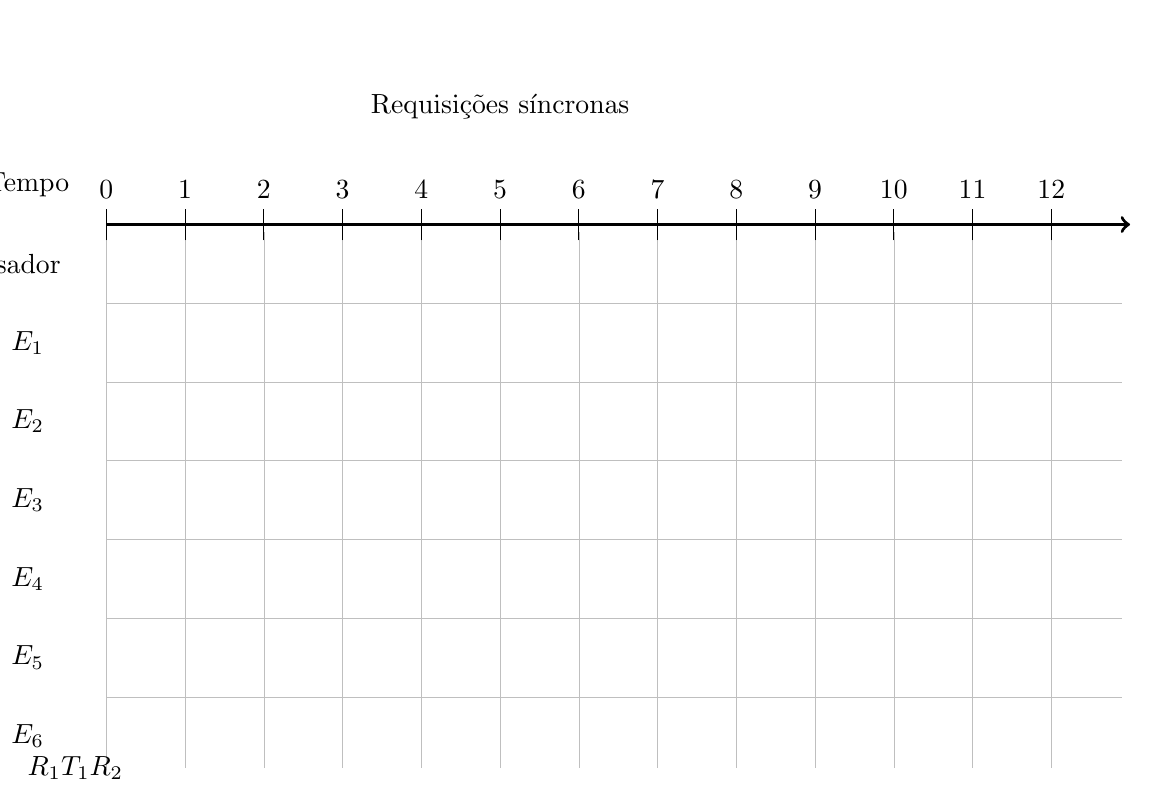
\begin{tikzpicture}
        \useasboundingbox (0,0) rectangle (14,9.5);
        \node at (6, 8.5) {Requisições síncronas};
        \draw[step=1cm,lightgray,very thin] (1,0.1) grid (13.9,6.9);
        \foreach \x in {0,1,2,3,4,5,6,7,8,9,10,11,12}
            \draw ((1cm+\x cm,6.8) -- (1cm+\x cm,7.2) node[anchor=south] {$\x$};
        \draw[very thick,->] (1,7) -- (14,7) node[anchor=south west] {};
        \node at (0,7.5) {Tempo};
        \node at (-0.5,6.5) {Processador};
        \foreach \i in {1,...,6}{
            \node at (0,6.5-\i) {$E_\i$};
        }
        \blocoR{0}{$R_1$}
        \blocoE{1}{1}{6}
        \blocoT{7}{$T_1$}
        \blocoR{8}{$R_2$}
        \blocoE{2}{9}{4}
    \end{tikzpicture}

    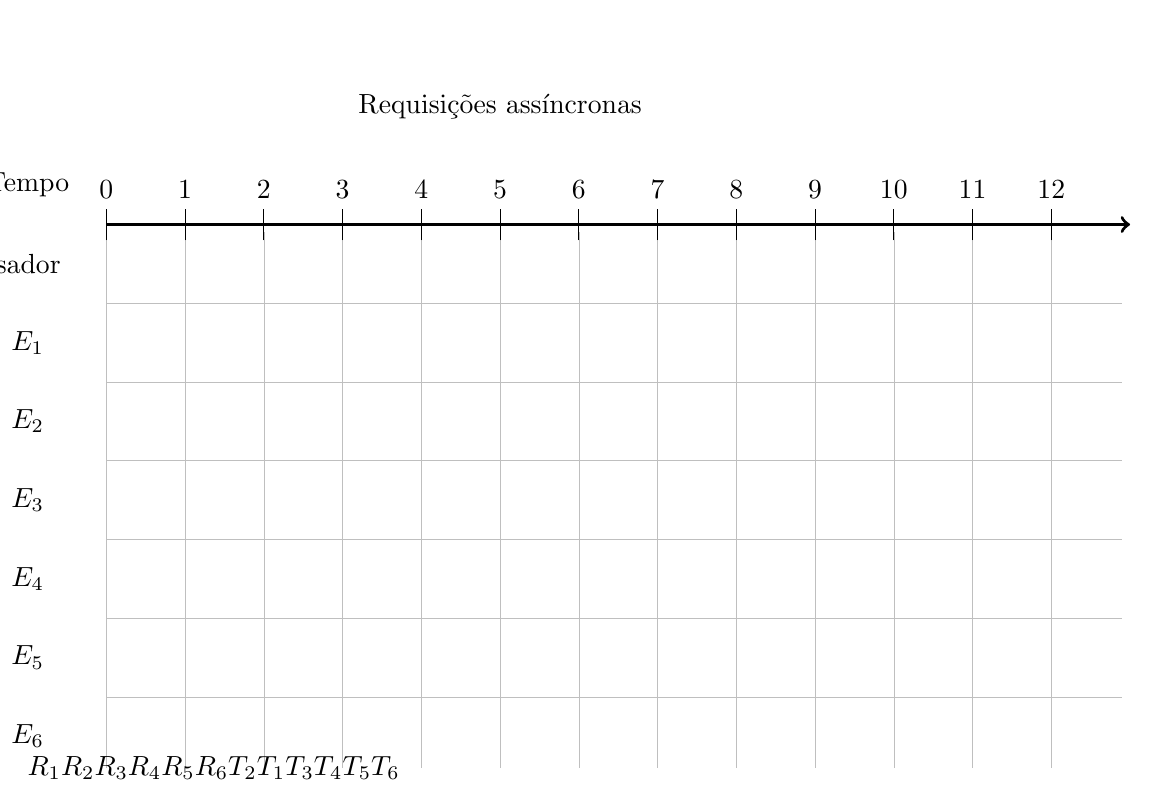
\begin{tikzpicture}
        \useasboundingbox (0,0) rectangle (14,9.5);
        \node at (6, 8.5) {Requisições assíncronas};
        \draw[step=1cm,lightgray,very thin] (1,0.1) grid (13.9,6.9);
        \foreach \x in {0,1,2,3,4,5,6,7,8,9,10,11,12}
            \draw ((1cm+\x cm,6.8) -- (1cm+\x cm,7.2) node[anchor=south] {$\x$};
        \draw[very thick,->] (1,7) -- (14,7) node[anchor=south west] {};
        \node at (0,7.5) {Tempo};
        \node at (-0.5,6.5) {Processador};
        \foreach \i in {1,...,6}{
            \node at (0,6.5-\i) {$E_\i$};
        }
        \foreach \i in {1,2,3,4,5,6}{
            \blocoR{\i-1}{$R_\i$};
        }
        \foreach \i [count=\n] in {2,1,3,4,5,6}{
            \blocoT{\n + 5}{$T_\i$};
        }
        \blocoE{1}{1}{6}
        \blocoE{2}{2}{4}
        \blocoE{3}{3}{4}
        \blocoE{4}{4}{5}
        \blocoE{5}{5}{5}
        \blocoE{6}{6}{5}
    \end{tikzpicture}
    \caption{%
        Comparativo ilustrando como seriam executadas as operações de envio,
        espera e tratamento das requisições enviadas ao servidor de um TJ
        hipotético considerando a obtenção dos dados de 6 processos, enumerados
        como $P_{1...6}$. A sequência das operações estão em passos de tempo
        discretos ordenados da esquerda para direita. A linha ``Processador''
        indica em qual operação o processador está trabalhando em um
        determinado passo de tempo e as linhas $E_{1...6}$ representam uma
        operação de IO relacionada a uma requisição $R_i$, como a espera pela
        resposta do servidor.
        %
        Para cada processo $P_i$, $R_i$ representa a operação de preparo e
        envio da requisição e $T_i$ representa a operação de tratamento da
        resposta do servidor do TJ a $R_i$ (por exemplo, classificação do
        processo como válido/inválido/inexistente ou reconhecimento de resposta
        com \textit{Captcha}).
    }
    \label{gra:modelo-temporização-requisições}
\end{figure}


\subsection{\textit{Cache} dos resultados}

\begin{todolist}
    \item Justificar a necessidade de \textit{cache} para os resultados: em
          resumo, requisições, sejam de um mesmo usuário ou de usuários
          diferentes, podem muito bem conter uma intersecção dos processos que
          serão buscados.
    \item Adicionar gráfico comparando o uso da cache para a mesma consulta com
          quando ela é feita com e sem caching.
\end{todolist}

Dado o tempo para realizar uma busca por todos os processos, é inviável que ela
reacesse o servidor dos TJs para cada consulta realizada na ferramenta. A
estratégia para atacar esse problema consiste em guardar os processos
previamente buscados em um banco de dados simples, funcionando como uma
\textit{cache} para os processos já conhecidos. A \textit{cache} acaba sendo
útil também para diferentes requisições em que seus intervalos de números de
processos se interseccionem, visto que a primeira requisição atendida já trará
alguns dos processos da(s) próxima(s), não precisando ser re-buscados por
requisições ao servidor do TJ-RJ já que estarão prontos no banco de dados da
ferramenta. Há também uma vantagem adicional com relação a descoberta de
processos válidos uma vez que, conhecidos todos os processos de um único ano,
não é necessário gastar tempo descobrindo quais números de processos
correspondem a processos reais.

A \textit{cache} foi implementada como um instância de banco de dados
SQLite~\cite{tool:sqlite} com uma única tabela ``Processos'' (reproduzida na
\Cref{tbl:estrutura-tabela-processos}), com a descrição dos valores possíveis
para a coluna \textit{``cache\_state''} descritos
na~\Cref{tbl:valores-coluna-state}. A chave primária da tabela foi escolhida
como o número do processo seguindo a numeração unificada, visto que é uma
informação única a cada processo e, convenientemente, é o parâmetro de busca
utilizado na extração, facilitando a separação de quais processos serão
buscados na \textit{cache} e quais serão requisitados ao servidores dos TJs.

\begin{table}[htb]
    \small
    \centering
    \begin{tabular}{llp{0.6\textwidth}}
        \toprule
        \multicolumn{3}{c}{Processos} \\
        \midrule
        Coluna & Tipo & Descrição \\
        \midrule \\
        *\texttt{id} & text & Número do processo no padrão unificado. \\
        \texttt{cache\_state} & text & Estado atual do processo na \textit{cache}. \\
        \texttt{assunto} & text & Assunto do processo. \\
        \texttt{json} & text & Dados do processo no formato JSON espelhando os campos retornados pela API do ww3. \\
        \bottomrule
    \end{tabular}
    \caption{%
        Definição da tabela SQLite ``Processos'' utilizada para \textit{cache}.
        ``*'' indica que o campo é uma chave primária.
    }
    \label{tbl:estrutura-tabela-processos}
\end{table}

\begin{table}[htb]
    \centering
    \begin{tabular}{lp{0.8\textwidth}}
        \toprule
        Estado & Descrição \\
        \midrule \\
        \texttt{CACHED} & O número do processo é válido e os dados do processo estão na \textit{cache}. \\
        \texttt{INVALID} & O número do processo é inválido (por exemplo, dígitos de validação não conferem pelo algoritmo do TJ). \\
        \texttt{NOT\_CACHED} & O número do processo é válido porém os dados dele não estão na \textit{cache}. Para uso no software, não é registrado na \textit{cache}. \\
        \bottomrule
    \end{tabular}
    \caption{%
        Definição da tabela SQLite ``Processos'' utilizada para \textit{cache}.
        ``*'' indica que o campo é uma chave primária.
    }
    \label{tbl:valores-coluna-state}
\end{table}

Essa separação é uma operação trivial: para saber se um processo deve ou não
ser requisitado aos servidores dos TJs, basta para cada número de processo da
lista de números a serem buscados consultar, na \textit{cache}, se não existe
uma entrada com esse número como valor da chave primária e que o valor de
``cache\_state'' seja ``CACHED''.

Um processo sempre é salvo na \textit{cache} quando o servidor do TJ responde à
requisição referente a uma consulta por número de processo, com exceção de
casos em que a resposta é um erro de captcha.

\todo{Falar sobre quando um processo é cacheado e quando não é}

\section{Estratégias adicionais}

\subsection{Filtragem dos resultados}
